
\section{Organisation}

\begin{frame}
  {Literatur | Einführungen}
  \onslide<+->
  \onslide<+->
  Die folgenden drei Bücher sind die Grundlage der Vorträge:\\
  \Zeile
  \begin{itemize}[<+->]
    \item \alert{\citet{ChierchiaMcconnellginet2000}} | GB-orientiert, nur die Kapitel von Chierchia
    \item \alert{\citet{DowtyEa1981}} | Tolle Montague-Einführung von seinen Schülern
    \item \alert{\citet{ParteeEa1990}} | Wichtige Grundlagen (Algebra, Logik), viele Druckfehler
  \end{itemize}
  \onslide<+->
  \centering 
  \large
  \Zeile
  \rot{Die auf den Folien angegebenen Teile dieser Bücher sollten\\
  für die Prüfungen durchgearbeitet werden. Das heißt natürlich nicht,\\
  dass Sie alles auswendig lernen sollen. Die Folien geben die Hinweise,\\
  was aus den Texten wichtig ist, sind aber nicht selbsterklärend.}
\end{frame}

\begin{frame}
  {Literatur | weitere Empfehlungen}
  \onslide<+->
  \begin{itemize}[<+->]
    \item \alert{\citet{Bucher1998}} | Lesbare Logik-Einführung auf Deutsch
    \item \alert{\citet{Carpenter1997}} | Prima Hardcore-Einführung mit Kategorialgrammatik
    \item \alert{\citet{Gutzmann2019}} | Aktuelle Einführung auf Deutsch
  \end{itemize}
\end{frame}


\begin{frame}
  {Semesterplan und Lernen für die Prüfung}
  \onslide<+->
  \onslide<+->
  \centering 
  \alert{\large Hinweis zum Lernen}\\
  \Halbzeile
  \begin{itemize}[<+->]
    \item Wir haben es hier mit anspruchsvollem Material zu tun.
    \item Nur so ergibt meiner Meinung nach formale Semantik Sinn,\\
      und irgendwelche weichgespülten Einführungen sind grob fahrlässig.
    \item Daher gilt aber: Wenn Sie nicht von Anfang an lernen,\\
      wird es sehr wahrscheinlich gegen Ende sehr schwierig!
  \end{itemize}
\end{frame}

\begin{frame}
  {Prüfungen}
  \onslide<+->
  \onslide<+->
  Einheitlicher Inhalt für alle Modul- und Examensprüfungen:\\
  \Zeile
  \begin{quote}
    Sie erhalten in der Prüfung zwei der Originaltexte zur Auswahl und müssen einen davon diskutieren und in den Seminarkontext einordnen. Dazu gibt es Leitfragen, über die ich auf Basis des Seminarverlaufs entscheide.
  \end{quote}
  \Zeile
  \onslide<+->
  \grau{Hausarbeiten nach Absprache.}
\end{frame}

\begin{frame}
  {Die unausweichliche Frage nach ein paar Wochen \visible<2->{| \rot{WTF???}}}
  \onslide<+->
  \onslide<+->
  \onslide<+->
  "`Wozu brauchen wir das denn?"'\\
  \Halbzeile
  \begin{itemize}[<+->]
    \item Nicht zu leugnende \alert{logische Eigenschaften von Sprache}
    \item Kleiner Einblick in deren \alert{technisch sehr aufwendige Beschreibung}
      \Halbzeile
    \item Wichtige Lernziele
      \begin{itemize}[<+->]
        \item Realistische Einschätzung \alert{eigener semantischer Intuitionen}
        \item Erkennen der \alert{Grenzen der Möglichkeiten von Logik} in der Analyse von Sprache
        \item Für zukünftige Forschende | \alert{Grundausbildung in formaler Semantik unabdinglich}
      \end{itemize}
  \end{itemize}
\end{frame}

\section{Schlussfolgern}

\begin{frame}
  {Was folgt logisch?}
  \onslide<+->
  \onslide<+->
  Fallen Ihnen logische Schlussfolgerungen aus diesen Aussagen ein?\\
  \Halbzeile
  \begin{itemize}[<+->]
    \item Das Semester hat begonnen.
    \item Olha hat einen sehr leichten ukrainischen Akzent.
    \item Entweder regnet es gerade, oder die Wasserleitung ist gebrochen.
    \item Es regnet, oder die Wasserleitung ist gebrochen. Es regnet seit zwei Stunden.
    \item Falls der Dänemark-Urlaub ausfällt, fahre ich eine Woche zu meinen Eltern.\\
      Der Dänemark-Urlaub fällt aus.
    \item Wenn es regnet, wird die Straße nass. Die Straße ist nicht nass.
    \item Es ist nicht der Fall, dass der WANG PC keine Festplatten unterstützt hat.
  \end{itemize}
\end{frame}

\begin{frame}
  {Folgt B aus A?} % Sätze
  \onslide<+->
  \begin{itemize}[<+->]
    \item A: Ein blauer Renault fährt auf der A9 Richtung Berlin.\\
      \alert{B: Ein Renault fährt auf der A9 Richtung Berlin.}
    \item A: Ich finde Geranien abstoßend.\\
      \alert{B: Ich habe schon mindestens einmal mindestens eine Geranie gesehen.}
    \item A: Der WANG PC ist nicht IBM-kompatibel.\\
      \alert{B: Es existiert mindestens ein WANG PC.}
    \item A: Alle Menschen sind intelligent.\\
      \alert{B: Horst Lichter ist intelligent.}
    \item A: Krister hat mir seinen Volvo Amazon verkauft.\\
      \alert{B: Irgendjemand hat seinen Volvo Amazon verkauft.}
  \end{itemize}
\end{frame}

\begin{frame}
  {Folgt B aus A?} % Lexik und Grammatik
  \begin{itemize}[<+->]\small
    \item A: Entweder regnet es, oder die Wasserleitung im Bad ist gebrochen, und die Wasserleitung im Bad ist gebrochen.\\
      \alert{B: Es regnet nicht.}
    \item A: Michelle hat uns den Dobermann für eine Woche zur Pflege überlassen.\\
      \alert{B: Der Dobermann wurde uns für eine Woche zur Pflege überlassen.}
    \item A: Jan glaubt, dass seine Sendung nicht abgesetzt wird.\\
      \alert{B: Jan glaubt nicht, dass seine Sendung abgesetzt wird.}
    \item A: Falls Dr.\ Kohl jetzt wieder Kanzler der BRD ist, gibt es vermutlich jeden Tag Pfälzer Saumagen zum Abendessen.\\
      \alert{B: Es gibt einen Kanzler der BRD.}
    \item A: Ein Mensch betritt den Raum.\\
      \alert{B: Es gibt mindestens einen Menschen.}
    \item A: Ein Mensch, der die Bibel gelesen hat, begeht im Durchschnitt nicht weniger Straftaten als andere.\\
      \alert{B: Es gibt mindestens einen Menschen.}
    \item A: \textit{We don't need no education.}\\
      \alert{B: Yes, you do! You just used a double negative.}
  \end{itemize}
\end{frame}

\begin{frame}
  {Folgt B aus A?} % Stories
  \onslide<+->
  \begin{itemize}[<+->]
    \item A: Herr Sailer fährt einen Golf. Alles, was einen Golf fährt, ist entweder menschlich oder eine AI, die auf Deep Learning basiert. Es gibt keine AI, die auf Deep Learning basiert, die einen Golf fährt.\\
      \alert{B: Es gibt mindestens einen Menschen.}
      \Halbzeile
    \item A: Es gibt an der Uni Göttingen mindestens einen Dozenten, der einen Golf fährt. Manfred ist Dozent an der Uni Göttingen und Radsportler. Sein Auto ist gerade in der Werkstatt. Jeder Dozent an der Uni Göttingen fährt entweder einen Golf oder ist kein Radsportler, falls sein Auto in der Werkstatt ist.\\
      \alert{B: Manfred fährt einen Golf.}
  \end{itemize}
\end{frame}

\begin{frame}
  {Logik}
  \onslide<+->
  \onslide<+->
  \centering 
  Versuchen Sie, eine Definition des Begriffs \alert{logische Schlussfolgerung} zu geben.\\
  \onslide<+->
  \Zeile
  Wann folgt eine Aussage aus einer oder mehreren anderen Aussagen?
\end{frame}

\begin{frame}
  {Inferenz | Abduktion}
  \onslide<+->
  \onslide<+->
  Entspricht oft der "`Alltagslogik"'. Suche nach \alert{spontan plausiblen Ursachen}.\\
  \Halbzeile
  \begin{itemize}[<+->]
    \item A: Der Verdächtige hat kein Alibi, aber ein Motiv.\\
      B: Der Verdächtige ist der Täter.
    \item Ich habe so einen komischen Husten, und die Infektionszahlen steigen wieder.\\
      B: Oh mein Gott, ich habe Covid!
    \item A: Es soll eine Impfpflicht eingeführt werden.\\
      B: George Soros und Bill Gates wollen uns Mikrochips einpflanzen.
    \item A: In Mikes Büro ist um 22 Uhr noch Licht.\\
      B: Mike bereitet seine Lehrveranstaltung für morgen vor.
  \end{itemize}
  \onslide<+->
  \centering 
  \Zeile 
  \orongsch{Hochgradig gefährlich, weil nicht formalisierbar und sehr bequem.}\\
  \alert{Gleichzeitig im Alltag unentbehrlich.}\\
  \grau{\footnotesize Die meisten "`logischen"' Schlussfolgerungen von Vulkaniern sind im besten Fall Abduktionen.}
\end{frame}

\begin{frame}
  {Inferenz | Induktion}
  \onslide<+->
  \onslide<+->
  Suche nach \alert{allgemeingültigen Aussagen} aus Partikularereignissen.\\
  \Halbzeile
  \begin{itemize}[<+->]
    \item A\Sub{1}: Im Zentrum der Galaxis befindet sich ein supermassives schwarzes Loch.\\
          A\Sub{2}: Die Galaxis ist eine Galaxie.\\
          B: Im Zentrum jeder Galaxie befindet sich ein supermassives schwarzes Loch.
    \item A: Im Zentrum von 1200 Galaxien befindet sich ein supermassives schwarzes Loch.\\
          B: Im Zentrum jeder Galaxie befindet sich ein supermassives schwarzes Loch.
    \item A: Aus dieser Einmündung kam noch nie ein Auto von rechts.\\
          B: Aus dieser Einmündung wird in drei Sekunden kein Auto von rechts kommen.
  \end{itemize}
  \onslide<+->
  \Zeile 
  \centering 
  \alert{"`Besser"' als Abduktion, vor allem je mehr Partikularereignisse zugrundeliegen.}\\
  \orongsch{Kann trotzdem gewaltig daneben gehen.}\\
  \grau{\footnotesize Spielt in der Wissenschaft eine große Rolle, aber ist fundamental nicht ausreichend.}
\end{frame}

\begin{frame}
  {Inferenz | Deduktion}
  \onslide<+->
  \onslide<+->
  \alert{Prämissen} (egal, wo diese herkommen) und formale \alert{Schlussregeln}\\
  \Halbzeile
  \begin{itemize}[<+->]
    \item A\Sub{1}: Manfred ist ein Dozent an der Uni Göttingen.\\
      A\Sub{2}: Jeder Dozent an der Uni Göttingen ist ein Mensch.\\
      B: Manfred ist ein Mensch.
    \item A\Sub{1}: Entweder (wurde die Welt von einem Gebrauchtwagenhändler erschaffen) oder (Rewe verkauft keine Weetabix).\\
      A\Sub{2}: Rewe verkauft keine Weetabix.\\
      B: Die Welt wurde von einem Gebrauchtwagenhändler erschaffen.
  \end{itemize}
  \onslide<+->
  \Zeile
  \centering 
  \alert{Nur Deduktion ist Logik. Nur darum geht es in diesem Semester.}
\end{frame}

\begin{frame}
  {Ganz trivial ist das nicht \ldots}
  \onslide<+->
  \onslide<+->
    A: Herr Sailer fährt einen Golf. Alles, was einen Golf fährt, ist entweder menschlich oder eine AI, die auf Deep Learning basiert. Es gibt keine AI, die auf Deep Learning basiert, die einen Golf fährt.\\
    \alert{B: Es gibt mindestens einen Menschen.}\\
    \onslide<+->
    \Halbzeile
    Hier ist der Beweis:\\
    \onslide<+->
    \Halbzeile
    \centering
    \scalebox{0.8}{\begin{tabular}[h]{rll}
      1  & $G(s)$                                          & \\
      2  & $(\forall x)[(G(x)\rightarrow M(x)\vee A(x)]$   & \\
      3  & $\neg(\exists y)[A(y)\wedge G(y)]$              & $\vdash(\exists z)M(z)$  \\
      \cline{1-3}
      4  & $(\forall y)\neg[A(y)\wedge G(y)]$              & 3,QN \\
      5  & $(\forall y)[\neg A(y)\vee\neg G(y)]$           & 4,DeM \\
      6  & $(\forall y)[G(y)\rightarrow \neg A(y)]$        & 5,Komm.,Impl. \\
      7  & $G(m)\rightarrow \neg A(m)$                     & 6,$-\forall(1)$ \\
      8  & $\neg A(m)$                                     & 1,7,MP \\
      9  & $G(m)\rightarrow M(m)\vee A(m)$                 & 2,$-\forall(1)$ \\
      10 & $M(m)\vee A(m)$                                 & 1,9,MP \\
      11 & $M(m)$                                          & 8,10,DS \\
      12 & $(\exists z)M(z)$                               & 11,$+\exists$ $\blacksquare$ \\
    \end{tabular}}
\end{frame}

\section{Grundfragen der Semantik}

\begin{frame}
  {Semantikbegriff in diesem Seminar}
  \onslide<+->
  \onslide<+->
  Es dreht sich alles um die Beziehung von Sprache zur Welt!\\
  \Zeile
  \begin{itemize}[<+->]
    \item Auf welche Klassen von Objekten \alert{referieren} welche Klassen von Ausdrücken?
    \item Wann sind Sätze wahr? (auch als Phänomen der \alert{Referenz}!)
    \item Wie verhält sich die logische Struktur von Sätzen zu ihrem Informationsgehalt?
    \item Wie können Sätze eindeutig interpretiert werden,\\
      auch wenn sie mehrere Lesarten haben?
  \end{itemize}
\end{frame}

\section{Programmatisches Schlussbild}

\begin{frame}
  {Programmatisches Schlussbild | Exkurs I}
  \onslide<+->
  \onslide<+->
  \alert{Kognition}\\
  \Viertelzeile
  \begin{itemize}[<+->]
    \item basierend auf Ähnlichkeiten von wahrgenommenen Objekten
    \item optimiert für schnelle Mustererkennung \alert{in allen Bereichen}
    \item unscharfe Klassenbildung und Segmentierung der Ontologie
    \item parallele Verarbeitung (meistens mehrere Areale beteiligt)
  \end{itemize}
  \Halbzeile 
  \onslide<+->
  \alert{Symbolische Systeme}\\
  \Viertelzeile
  \begin{itemize}[<+->]
    \item diskrete Symbole, wohldefinierte Semantik
    \item scharf getrennte Klassen von Symbolen
    \item eindeutige Referenz auf ontologische Objekte
    \item intrinsische (nicht emergente) logische Eigenschaften\\
      \grau{(Axiomatik, Schlussregeln usw.)}
    \item sequentielle Verarbeitung\slash statische Deklaration\\
      \grau{(\zB Python oder PROLOG; parallele Verarbeitung immer linearisierbar)}
  \end{itemize}
\end{frame}

\begin{frame}
  {Programmatisches Schlussbild | Exkurs II}
  \onslide<+->
  \onslide<+->
  Klassisches kognitives Modell: \alert{Prototypentheorie} \grau{\citep{Rosch1973}}\\
  \onslide<+->
  \Zeile
  \alert{Diskretes Symbol}: \gruen{Vogel} \onslide<+-> \ldots\ und demgegenüber \ldots\\
  \onslide<+->
  \alert{Graduelles kognitives Konzept} basierend auf Ähnlichkeiten\slash Prototypen:\\
  \onslide<+->
  \Halbzeile
  \begin{minipage}{0.9\textwidth}
  \centering
    $\vcenter{\hbox{\includegraphics[width=0.4\textwidth]{\GRAPHPATH/spatz}}}$
    \onslide<+->
    \hspace*{0.025\textwidth}>\hspace*{0.025\textwidth}
    $\vcenter{\hbox{\includegraphics[width=0.25\textwidth]{\GRAPHPATH/kolibri}}}$
    \onslide<+->
    \hspace*{0.025\textwidth}>\hspace*{0.025\textwidth}
    $\vcenter{\hbox{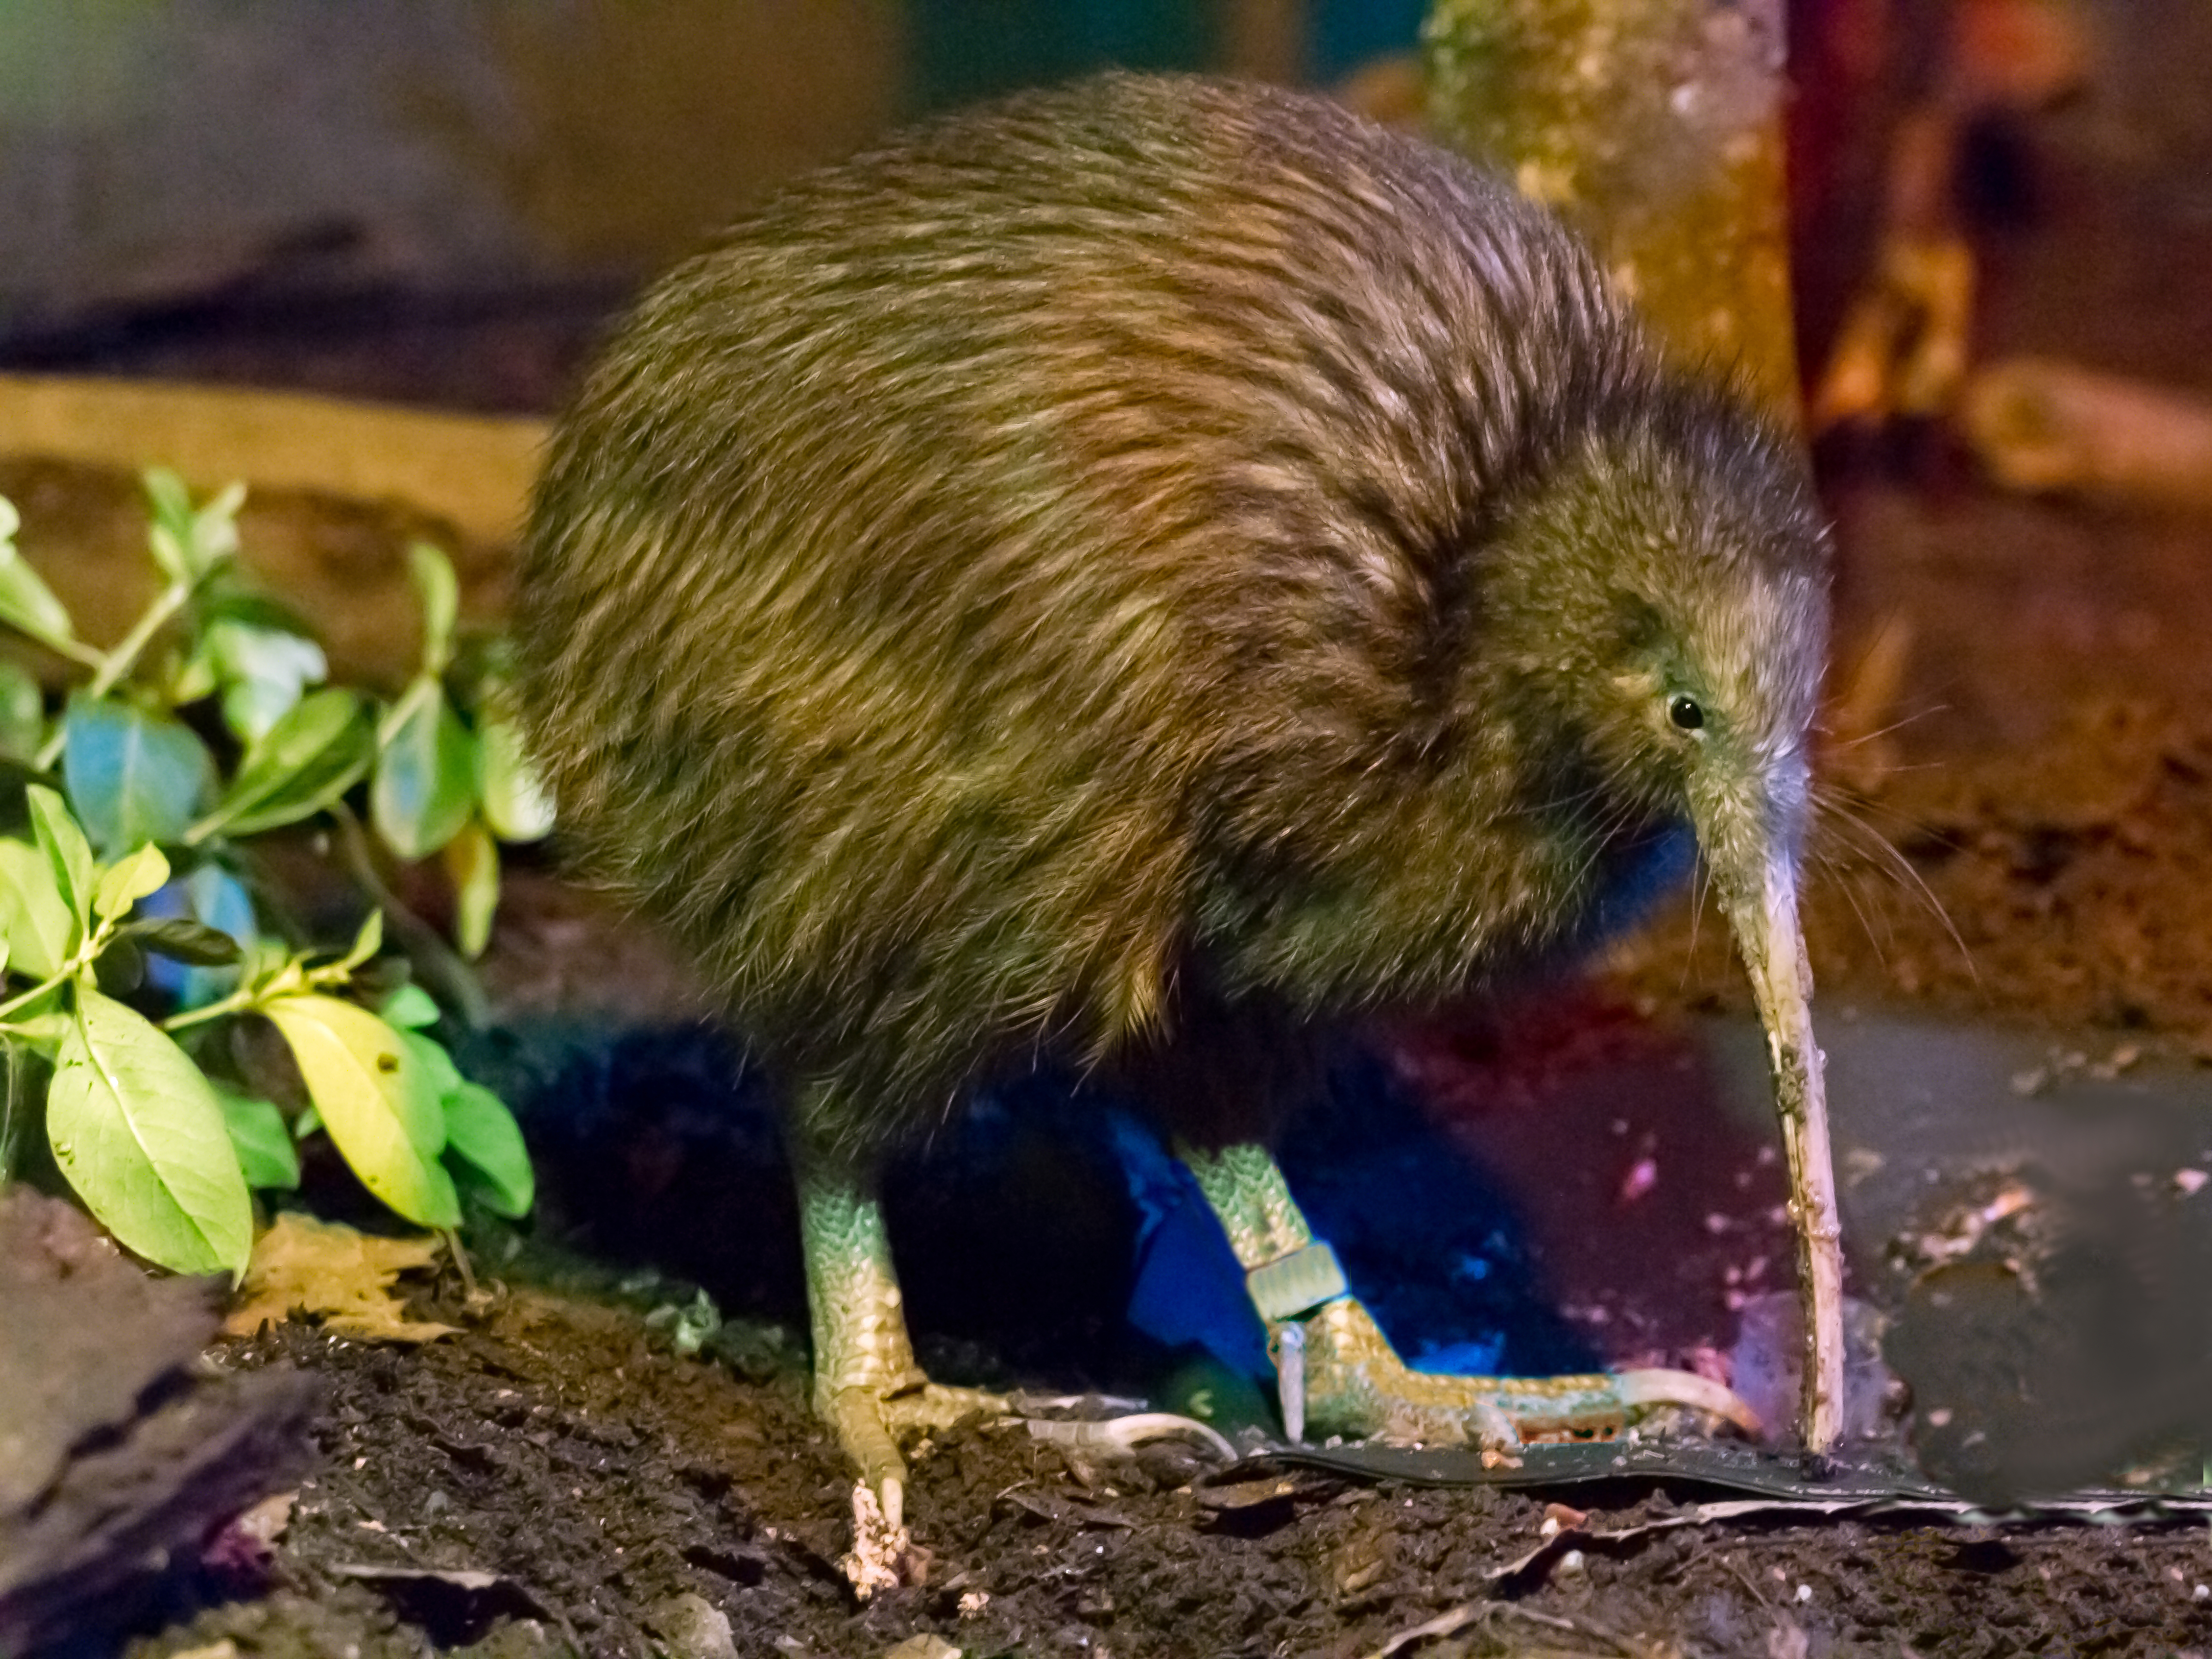
\includegraphics[width=0.1\textwidth]{\GRAPHPATH/kiwi}}}$
  \end{minipage}\\
  \Halbzeile
  \centering 
  \grau{\tiny Bildquelle: Wikipedia}
\end{frame}

\begin{frame}
  {Programmatisches Schlussbild | Antwort}
  \onslide<+->
  \onslide<+->
  Die ewige Schwachsinnsfrage: Sind Kiwis und Pinguine nun \gruen{Vögel} oder nicht?\\
  \Viertelzeile
  \grau{Nur getoppt von: Erdbeeren sind gar keine Beeren, sondern Sammelnussfrüchte.}\\
  \Zeile
  \begin{itemize}[<+->]
    \item \alert{Kognition} | \orongsch{intrinsisch nicht diskret}, sondern ähnlichkeitsbasiert und \orongsch{parallel}
      \begin{itemize}[<+->]
        \item \orongsch{Netzwerkarchitektur}
      \end{itemize}
      \Halbzeile
    \item \alert{Symbole} = Phone, Morphe, Wörter, Phrasen, \ldots | \orongsch{intrinsisch} diskret und \orongsch{linear}
      \begin{itemize}[<+->]
        \item \orongsch{akustisches} Medium | Sagen Sie mal zwei Wörter gleichzeitig!
        \item \orongsch{schriftliches} Medium | Lesen Sie mal \textit{Zettels Traum} von Arno Schmidt\\
          \grau{(inkl.\ der Versuche, mehrere Wörter "`in einem"' zu schreiben)}
      \end{itemize}
    \Halbzeile
    \item[\ding{222}] Da wir nur akustisch oder über schriftliche Artefakte kommunizieren können,\\
      \alert{muss das Sprachsystem symbolisch sein}.
    \item[\ding{222}] Da es architekturbedingt nur nicht-symbolisch verarbeiten kann,\\
      \alert{muss das Gehirn symbolische Systeme so gut wie nötig und möglich emulieren}.
  \end{itemize}
\end{frame}


\begin{frame}
  {Programmatisches Schlussbild | Ausführung}
  \onslide<+->
  \onslide<+->
  Auch nicht-verschriftete Sprache muss medial bedingt logische Eigenschaften haben.\\
  \onslide<+->
  Kulturell bilden sich stärker symbolische Modi aus, vor allem durch Schrift.\\
  \grau{\footnotesize Norm, Selbst- und Fremdkorrektur, Textplanung, intensionale Definitionen, Explizierung, \ldots}\\
  \grau{\footnotesize Warum wird das vor allem im Kontext von Schule, Fremdsprache und Bildungssprache diskutiert?}\\
  \onslide<+->
  \Zeile
  \Halbzeile
  \centering 
  \begin{tabular}[h]{cc}
    \grau{(= spontane Sprachproduktion)} & \\
    \orongsch{weniger symbolische Eigenschaften} & \small \orongsch{informelle Alltagssprache} \\
    \onslide<+->
    \textcolor{orgrA}{\faArrowDown} &\large \textcolor{orgrA}{formelle Alltagssprache} \\
    \onslide<+->
    \textcolor{orgrB}{\faArrowDown} &\Large \textcolor{orgrB}{Bildungssprache} \\
    \onslide<+->
    \textcolor{orgrC}{\faArrowDown} &\LARGE \textcolor{orgrC}{Wissenschaftssprache} \\
    \onslide<+->
    \textcolor{orgrD}{\faArrowDown} &\huge \textcolor{orgrD}{Orthosprache} \\
    \onslide<+->
    \gruen{mehr symbolische Eigenschaften} & \gruen{\Huge formales System} \\
    \grau{(= reflektierte Sprachproduktion)}  & \\
  \end{tabular}
\end{frame}

\ifdefined\HANDOUT
  \begin{frame}
    {Und was ist denn nun mit Kiwis und Pinguinen?}
    \onslide<+->
    \onslide<+->
    Unser Verständnis der Welt führt zu genaueren und diskreten Kategorisierungen,\\
    \orongsch{wo dies nötig ist}. \alert{Die Sprache folgt dem erforderlichen Maß an Genauigkeit\slash Diskretheit.}\\
    \Zeile
    \onslide<+->
    \centering
    \begin{tikzpicture}
      \node at (0cm, 0cm) {\includegraphics[height=0.6\textheight]{\GRAPHPATH/birds50}};
      \node at (5cm, 1.5cm) {\includegraphics[height=0.25\textheight]{\GRAPHPATH/kiwis}};
      \node at (5cm, -1.5cm) {\includegraphics[height=0.25\textheight]{\GRAPHPATH/penguins}};
      \path (-0.3cm, 2.5cm) edge [-latex] (4.6cm, 1.25cm);
      \path (1.1cm, -0.45cm) edge [-latex] (4.2cm, -1.725cm);
    \end{tikzpicture}\\
    \Halbzeile
    \grau{\tiny Bildquelle: Wikipedia}
  \end{frame}
\else
  \begin{frame}
    {Und was ist denn nun mit Kiwis und Pinguinen?}
    \onslide<+->
    \onslide<+->
    Unser Verständnis der Welt führt zu genaueren und diskreten Kategorisierungen,\\
    wo dies nötig ist. \alert{Die Sprache folgt diesem Maß an Genauigkeit und Diskretheit!}\\
    \Zeile
    \onslide<+->
    \centering
    \begin{minipage}{0.9\textwidth}
    \centering
      $\vcenter{\hbox{\includegraphics[height=0.7\textheight]{\GRAPHPATH/birds50}}}$\hspace{0.1\textwidth}
        \only<3>{$\vcenter{\hbox{\rule{0.4\textwidth}{0em}}}$}%
        \only<4>{$\vcenter{\hbox{\includegraphics[width=0.4\textwidth]{\GRAPHPATH/kiwis}}}$}%
        \only<5>{$\vcenter{\hbox{\includegraphics[width=0.4\textwidth]{\GRAPHPATH/penguins}}}$}
    \end{minipage}\\
    \grau{\tiny Bildquelle: Wikipedia}
  \end{frame}
\fi


\section{Linguistische Theorien}

\begin{frame}
  {"`Semantik"' im generativen T-Modell}
  \onslide<+->
  \onslide<+->
  \centering 
  \resizebox{0.6\textwidth}{!}{
    \begin{tikzpicture}

      \node [rectangle, draw, align=left, color=teal, rounded corners=0.5em] (Numeration) at (5cm, -6cm) {Numeration};
      
      \node [visible on=<3->, rectangle, draw, align=left, color=gray] (Lexikon) at (1cm, -6cm) {Lexikon};
      \path (Lexikon.east) edge [visible on=<3->, line width=0.5mm, dashed] node [below, shift={(-0.4cm,0)}] {\textit{}} (Numeration.west);
     
      \node [visible on=<4->, rectangle, draw, align=left, color=gray] (Intention) at (9cm, -6cm) {Intention};
      \path (Intention.west) edge [visible on=<4->, line width=0.5mm, dashed] node [below, shift={(-0.4cm,0)}] {\textit{}} (Numeration.east);

      \node [visible on=<5->, rectangle, draw, align=left, fill=black, color=black, rounded corners=0.5em] (Syntax) at (5cm, -4.5cm) {\whyte{Syntax}};
      \path (Numeration.north) edge [visible on=<5->, line width=0.5mm, -latex] node [below, shift={(-0.4cm,0)}] {\textit{}} (Syntax.south);  

      \node [visible on=<6->, rectangle, draw, align=left, color=teal, rounded corners=0.5em] (Phrasenstruktur) at (5cm, -3cm) {Phrasenstruktur};
      \path (Syntax.north) edge [visible on=<6->, line width=0.5mm, -latex] node [below, shift={(-0.4cm,0)}] {\textit{}} (Phrasenstruktur.south);  

      \node [visible on=<7->, rectangle, draw, align=left, color=teal, rounded corners=0.5em] (PF) at (4cm, 0cm) {PF};
      \path (Phrasenstruktur.north) edge [visible on=<7->, line width=0.5mm, -latex] node [below, shift={(-0.4cm,0)}] {\textit{}} (PF.south);  
     
      \node [visible on=<8->, rectangle, draw, align=left, color=gray] (Aeusserung) at (1cm, 0cm) {Äußerung};
      \path (Aeusserung.east) edge [visible on=<8->, line width=0.5mm, dashed] node [below, shift={(-0.4cm,0)}] {\textit{}} (PF.west);
     
      \node [visible on=<9->, rectangle, draw, align=left, fill=black, color=black, rounded corners=0.5em] (Syntax2) at (6cm, -1.5cm) {\whyte{Syntax 2}};
      \path (Phrasenstruktur.north) edge [visible on=<9->, line width=0.5mm, -latex] node [below, shift={(-0.4cm,0)}] {\textit{}} (Syntax2.south);  
     
      \node [visible on=<10->, rectangle, draw, align=left, color=teal, rounded corners=0.5em] (LF) at (6cm, 0cm) {LF};
      \path (Syntax2.north) edge [visible on=<10->, line width=0.5mm, -latex] node [below, shift={(-0.4cm,0)}] {\textit{}} (LF.south);  

      \node [visible on=<11->, rectangle, draw, align=left, color=gray] (Interpretation) at (9cm, 0cm) {Interpretation};
      \path (Interpretation.west) edge [visible on=<11->, line width=0.5mm, dashed] node [below, shift={(-0.4cm,0)}] {\textit{}} (LF.east);
      
    \end{tikzpicture}
  }
\end{frame}

\begin{frame}
  {Repräsentationsebenen}
  \onslide<+->
  \onslide<+->
  Im klassischen generativen Modell:\\
  \grau{\footnotesize (In minimalistischen Modellen herrscht -- Chomsky muss es mögen! -- sowieso Anarchie.)}
  \Zeile
  \begin{itemize}[<+->]
    \item keine echte Interpretation auf LF
    \item Bewegung \rot{nachdem} der Satz geäußert wurde
    \item Herstellung einer logisch interpretierbaren \alert{Form} auf LF
    \item Grund | Syntax kann nicht alle Interpretationen abbilden
      \Halbzeile
      \begin{itemize}[<+->]
        \item[ ] \alert{Klassiker Quantorenskopus}
        \item[ ] \textit{Everybody loves somebody.}
          \Viertelzeile
        \item[A] Für alle Personen y gilt, dass es eine Person x gibt, für die gilt: y liebt x \grau{| $(\forall y)(\exists x)L(y,x)$}
        \item[B] Es gibt eine Person x, sodass für alle Personen y gilt: y liebt x \grau{| ($\exists x)(\forall y)L(y,x)$}
      \end{itemize}
  \end{itemize}
\end{frame}


\begin{frame}
  {Montagues direkte Interpretation}
  \onslide<+->
  \onslide<+->
  Sprache ist Logik ist Sprache \ldots\\
  \Halbzeile
  \begin{itemize}[<+->]
    \item[A] Entweder ist die \alert{Übersetzung in eine LF trivial und äquivalent zur PF\slash Syntax},\\
      oder \orongsch{sie fügt etwas hinzu, das der Sprache an sich fehlt}.
    \item[B] Sätze haben aber auch \alert{mit LF-Übersetzung nur die Bedeutungen,\\
      die sie sowieso haben} \grau{(keine Hinzufügung)}.
    \item[\ding{222}] Also ist die \gruen{Übersetzung in LF trivial und äquivalent zur PF\slash Syntax}.
    \item[\ding{222}] Wir können \gruen{Sätze direkt interpretieren} (wie sie gesprochen\slash geschrieben werden).
     \Zeile 
   \item \alert{Montagues \textit{lf}} | direkte Übersetzung von sprachlichen in logische Ausdrücke
  \end{itemize}
\end{frame}

\section{Referentielle Semantik basal}

\begin{frame}
  {Interessante Eigenschaften von Sprache}
  \onslide<+->
  \begin{itemize}[<+->]
    \item Aussagen über die\slash Teile der Welt
    \item Ausdrücke bezeichnen\slash referieren auf Dinge i.\,w.\,S.
    \item Informativität
    \item objektiv beurteilbar (\zB Wahrheit von Sätzen)
      \Zeile
    \item \alert{Aber welche sprachlichen Einheiten referieren auf was?}
  \end{itemize}
\end{frame}

\begin{frame}
  {Referenz | Eigennamen}
  \onslide<+->
  \onslide<+->
  Ein \alert{Eigenname} \ding{222} \alert{genau ein Objekt} in der Welt\\
  \onslide<+->
  \Zeile
  \centering
    \begin{tikzpicture}
      \node [] (name) at (-6cm, 0cm) {\textit{Jan Böhmermann}};
      \node [visible on=<4->] (boehmi) at (0cm, 0cm) {
\includegraphics[width=0.2\textwidth]{\GRAPHPATH/boehmermann}};
      \path (name.east) edge [visible on=<4->, line width=0.5mm, -latex] node {\textit{}} (boehmi.west);
    \end{tikzpicture}
\end{frame}

\begin{frame}
  {Referenz | Appellativa}
  \onslide<+->
  \onslide<+->
  Ein normales \alert{Nomen} \ding{222} \alert{eine Menge von Objekten} in der Welt\\
  \onslide<+->
  \Zeile
  \centering
    \begin{tikzpicture}
      \node [] (noun) at (-6cm, 0cm) {\textit{soldier}};
      \node [visible on=<4->] (soldiers) at (0cm, 0cm) {\includegraphics[width=0.2\textwidth]{\GRAPHPATH/soldiers}};
      \path (noun.east) edge [visible on=<4->, line width=0.5mm, -latex] node {\textit{}} (soldiers.west);
    \end{tikzpicture}
\end{frame}

\begin{frame}
  {Referenz | Adjektive und Verben}
  \onslide<+->
  \onslide<+->
  Ein (intersektives) \alert{Adjektiv} oder ein \alert{Verb} \ding{222} \alert{eine Menge von Objekten} in der Welt\\
  \onslide<+->
  \Zeile
  \centering
    \begin{tikzpicture}
      \node [] (adj) at (-6cm, 0cm) {\textit{human}};
      \node [visible on=<4->] (boehmi) at (0cm, +2cm) {
\includegraphics[width=0.1\textwidth]{\GRAPHPATH/boehmermann}};
      \path (adj.east) edge [visible on=<4->, line width=0.5mm, -latex] node {\textit{}} (boehmi.west);
      \node [visible on=<5->] (soldiers) at (0cm, 0cm) {\includegraphics[width=0.1\textwidth]{\GRAPHPATH/soldiers}};
      \path (adj.east) edge [visible on=<5->, line width=0.5mm, -latex] node {\textit{}} (soldiers.west);
      \node [visible on=<6->] (crowd) at (0cm, -2cm) {\includegraphics[width=0.1\textwidth]{\GRAPHPATH/crowd}};
      \path (adj.east) edge [visible on=<6->, line width=0.5mm, -latex] node {\textit{}} (crowd.west);
    \end{tikzpicture}
\end{frame}

\begin{frame}
  {Referenz | Sätze}
  \onslide<+->
  \onslide<+->
  Ein \alert{Satz} \ding{222} in erster Näherung \alert{ein Sachverhalt}\\
  \onslide<+->
  \Zeile
  \centering
    \begin{tikzpicture}
      \node [align=left] (s) at (-6cm, 0cm) {\it A humming bird\\\it is hovering over\\\it a red flower.};

      \node [visible on=<4->, align=center] (hum) at (0cm, +2cm) {\includegraphics[width=0.2\textwidth]{\GRAPHPATH/hummingbird}};
      \path (s.east) edge [visible on=<4->, line width=0.5mm, -latex] node {\textit{}} (hum.west);
      
      \node [visible on=<5->, align=center] (boehmi) at (0cm, -2cm) {
\includegraphics[width=0.2\textwidth]{\GRAPHPATH/boehmermann}\\\footnotesize (als Individuum)};
      \path (s.east) edge [visible on=<5->, line width=0.5mm, -latex, color=red] node {\textit{}} (boehmi.west);
      \node [visible on=<6->, align=center, color=red, fill=red] (nein) at (-3.5cm, -1.25cm) {\footnotesize \whyte{Nein! falsche}\\\footnotesize \whyte{Art von Objekt}};
    \end{tikzpicture}
\end{frame}

\begin{frame}
  {Freges Prinzip | Das hier wollen wir formalisieren!}
  \onslide<+->
  \onslide<+->
  Bedeutung ist kompositional!\\
  \Halbzeile
  \begin{itemize}[<+->]\small
    \item \textit{humming bird} \ding{222} die \alert{Menge} der Kolibri-Objekte
    \item \textit{a} \ding{222} \alert{Existenzaussage} für ein Element aus einer Menge
    \item \textit{a humming bird} \ding{222} \alert{Existenzaussage} für ein Element $x$\\
      aus der Menge der Kolibri-Objekte
    \item \textit{is hovering} \ding{222} die \alert{Menge} der schwebenden Objekte
    \item \textit{a humming bird is hovering} \ding{222} das existierende Kolibri-Objekt $x$\\
      ist auch ein \alert{Element der Menge} der schwebenden Objekte
    \item \textit{a red flower} \ding{222} \alert{Existenzaussage} für ein Element $y$\\
      aus der \alert{Schnittmenge} der roten Objekte und der Blumen-Objekte
    \item \textit{over} \ding{222} die \alert{Relation} zwischen Objekten (s.\ nächste Woche),\\
      die sich übereinander befinden
    \item \textit{A Humming is hovering over a red flower.} \ding{222}\\
      \gruen{Es gibt ein Objekt $x$ aus der Schnittmenge der Kolibri- und der schwebenden Objekte,\\
      und es gibt ein Objekt $y$ aus der Schnittmenge der roten und der Blumen-Objekte,\\
    und $x$ befindet sich über $y$.}
  \end{itemize}
\end{frame}

\section{Semantische Eigenschaften von Sätzen}

\begin{frame}
  {Implikation (Entailment)}
  \onslide<+->
  \onslide<+->
  Mengen von Aussagesätzen \alert{implizieren} andere Sätze.\\
  \onslide<+->
  Sätze (Implikationen) lassen sich aus anderen Sätzen (Axiome) \alert{beweisen}.\\
  \Halbzeile
  \begin{itemize}[<+->]
    \item[A] \textit{Jan Böhmermann ist ein Mensch.}
    \item[B] \textit{Jan Böhmermann ist leutselig.}
    \item[C] \textit{Jan Böhmermann ist ein leutseliger Mensch.}
      \Halbzeile
    \item[ ] \alert{$A,B\vdash C$} | A und B implizieren C. (C ist beweisbar aus A und B.)
    \item[ ] \rot{$A\not\vdash C$} | A impliziert nicht C.
    \item[ ] \rot{$B\not\vdash C$} | B impliziert nicht C.
      \Halbzeile
    \item[ ] \orongsch{$A\vdash A\wedge A$} \onslide<+->| \textit{Jan Böhmermann ist ein Mensch \orongsch{und} Jan Böhmermann ist ein Mensch.}
      \Halbzeile
    \item[D] \textit{Irgendetwas ist ein Mensch.}
    \item[ ] \alert{$A\vdash D$} 
  \end{itemize}
\end{frame}

\begin{frame}
  {Tests auf Implikation}
  \onslide<+->
  \onslide<+->
  Wenn diese Kriterien zutreffen, impliziert A B:\\
  \Zeile
  \begin{itemize}[<+->]
    \item Wenn A wahr ist, ist B auch immer wahr.
    \item Eine Situation, die von B beschrieben wird, wird auch von A beschrieben.
    \item Die Information in B ist vollständig in der Information in A enthalten.
    \item Man kann unter keinen Umständen sagen: \textit{A ist wahr, aber B ist nicht wahr.}
  \end{itemize}
\end{frame}

\begin{frame}
  {Übung | Sind das Implikationen?}
  \begin{itemize}[<+->]\small
    \item Böhmermann ist Showmaster. $\vdash$ Böhmermann ist menschlich.
    \item Böhmermann ist nicht sehr groß. $\vdash$ Irgendjemand ist nicht sehr groß.
    \item Böhmermann ist nicht sehr groß. $\vdash$ Irgendjemand ist sehr groß.
    \item Manche Menschen sind leutselig. $\vdash$ Böhmermann ist leutselig.
    \item Ich habe das neue drip-133-Album gehört. $\vdash$ drip-133 hat ein neues Album veröffentlicht.
    \item Nachdem ich einen Sherry getrunken habe, habe ich den Kondensator getauscht.\\
      $\vdash$ Ich habe einen Sherry getrunken.
    \item Nachdem Linux nicht mehr startete, habe ich einen weiteren Sherry getrunken.\\
      $\vdash$ Linux ist noch nie gestartet.
    \item Mein ehemaliger Mitbewohner mag Becks.\\
      $\vdash$ Mein ehemaliger Mitbewohner könnte Sherry mögen.
    \item Böhmermann hat das heutige ZDF Magazin beendet.\\
      $\vdash$ Das heutige ZDF Magazin wurde beendet.
  \end{itemize}
\end{frame}

\begin{frame}
  {Synonymie}
  \onslide<+->
  \onslide<+->
  Synonyme Ausdrücke haben \orongsch{exakt} \alert{die gleiche Referenz}.\\
  \Halbzeile
  \begin{itemize}[<+->]
    \item lexikalische Synonymie | \textit{humming bird} $\stackrel{lex}{\equiv}$ \textit{colibri}
      \Halbzeile
    \item kompositionale Synonymie
      \begin{itemize}[<+->]
        \item[ ] \textit{Mulder traf seine entführte Schwester, nachdem er\\
          in die geheime Militärbasis eingebrochen war.}
        \item[$\equiv$] \textit{Bevor er seine entführte Schwester traf,\\
          brach Mulder in die geheime Militärbasis ein.}
      \end{itemize}
    \Halbzeile
    \item \alert{$A\equiv B\ \text{gdw}\ A\vdash B\ \text{und}\ B\vdash A$} (gegenseitige Implikation)
    \item \grau{\textit{gdw} = \textit{genau dann wenn} | \textit{iff} = \textit{if and only if}}
  \end{itemize}
\end{frame}

\section{Referenz von Sätzen}

\begin{frame}
  {Natürliche Sprache und Implikation}
  \onslide<+->
  \onslide<+->
  Referentielle Semantik \orongsch{modelliert mehr als} \alert{einfaches Zeigen auf Objekte durch Sprache}.\\
  \Viertelzeile
  \onslide<+->
  Zusätzliche Logik für Fälle wie diesen (und viele andere):\\
  \Zeile
  \onslide<+->
  \begin{tabular}[h]{lll}
    & \alert{\textit{Die Lieblingsblume meines Kolibris}} & \textit{ist rot.} \\
    \visible<6->{\orongsch{$\vdash$}} & \visible<5->{\alert{\textit{Eine Blume}} & \textit{ist rot.}} \\
  \end{tabular}
\end{frame}

\begin{frame}
  {Synonyme NPs}
  \onslide<+->
  \begin{itemize}[<+->]
    \item[a] \textit{colibri}
    \item[b] \textit{humming bird}
    \item[ ] \gruen{$a\stackrel{lex}{\equiv} b$}
      \Halbzeile
    \item[c] \textit{a brunette lady}
    \item[d] \textit{a brown-haired dame}
    \item[ ] \gruen{$c\equiv d$}
      \Halbzeile
    \item[e] \textit{the primates}
    \item[f] \textit{the apes and humans}
    \item[ ] \gruen{$e\equiv f$}
  \end{itemize}
\end{frame}

\begin{frame}
  {Ausgelassen: The Slingshot Argument}
  \onslide<+->
  \onslide<+->
  Das \textit{Slingshot Argument}:
  \begin{itemize}[<+->]
    \item Alle wahren Sätze haben dieselbe Bedeutung (1).
    \item Alle falschen Sätze haben dieselbe Bedeutung (0).
    \item Diese Bedeutung ist ihr \alert{Wahrheitswert}.
    \item In ausformulierten Semantiken ist das ihr \alert{Extension}.
    \item Die mehr ``inhaltliche'' Bedeutung eines Satzes\\
      wird dann als seine \alert{Intension} modelliert.
  \end{itemize}
  \Halbzeile
  \centering 
  \onslide<+->
  \grau{\scriptsize Der Beweis ist komplexer, s.\ \citet{Church1948}.\\
    Etwas zugänglicher in \url{https://plato.stanford.edu/entries/truth-values/slingshot-argument.html}}
\end{frame}

\begin{frame}
  {Synonymie von Konstituenten und Sätzen}
  Synonymie von Konstituenten im Satzkontext \ding{222} Satzsynonymie\\
  \onslide<+->
  \Halbzeile
  \begin{itemize}[<+->]
    \item[A] \alert{\textit{A \orongsch{colibri} is hovering over a red flower.}}
    \item[B] \alert{\textit{A \orongsch{humming bird} is hovering over a red flower.}}
    \item[ ] \gruen{$A\equiv B$ weil $a\equiv b$ und Satzkontext identisch}
    \item[ ] \gruen{$[\Sub{A} a]\equiv[\Sub{B} b]$ wenn $a\equiv b$ und $[\Sub{A} \_]=[\Sub{B} \_]$}
      \Halbzeile
    \item[C] \alert{\textit{Lauren Bacall was \orongsch{a brunette lady}.}}
    \item[D] \alert{\textit{Lauren Bacall was \orongsch{a brown-haired dame}.}}
    \item[ ] \gruen{$C\equiv D$ weil $c\equiv d$ und Satzkontext identisch}
      \Halbzeile
    \item[E] \alert{\textit{\orongsch{Primates} are intelligent.}}
    \item[F] \alert{\textit{\orongsch{The apes and humans} are intelligent.}}
    \item[ ] \gruen{$E\equiv F$ weil $e\equiv f$ und Satzkontext identisch}
  \end{itemize}
\end{frame}

\section{Reden in Fragmenten}

\begin{frame}
  {Grammatik- und Semantikfragmente}
  \onslide<+->
  \onslide<+->
  \alert{Konstruktive}, \alert{schrittweise} Annäherungen an sprachliche Modellierung\\
  \Zeile
  \begin{itemize}[<+->]
    \item Grammatikfragment | Ausschnitt einer Gesamtgrammatik
    \item erwünschte schrittweise Erweiterung von Fragmenten (vgl.\ HPSG)
      \Zeile
    \item Konstruktion eines Semantik-Fragments
      \begin{itemize}[<+->]
         \item grammatische Kategorien und Referenzen von Wörtern
         \item Grammatikmechanismen und zugehörige Bedeutungskonstruktion
         \item Ergebnis | Semantik von Sätzen und Beitrag aller Konstituenten dazu
      \end{itemize}
    \item \Halbzeile
      \alert{T-Sätze}
      \begin{itemize}[<+->]
        \item \alert{L} eine Sprache, \alert{S} ein Satz, \alert{v} ein Sachverhalt, \alert{p} eine Aussage über Wahrheitsbedingungen
        \item \alert{S aus L ist wahr in v gdw p.}
      \end{itemize}
  \end{itemize}
\end{frame}

\begin{frame}
  {Das Lexikon}
  \onslide<+->
  \onslide<+->
  Die folgenden simplexen Ausdrücke sind Teil von F\Sub{1}.\\
  \onslide<+->
  Kein anderer simplexer Ausdruck ist Teil von F\Sub{1}.\\
  \Halbzeile
  \begin{enumerate}[<+->]
    \item N $\rightarrow$ \emph{Herr Webelhuth, Frau Klenk, the Turm-Mensa} \label{lex01}
    \item V\Sub{{i}} $\rightarrow$ \emph{is relaxed, is creative, is stupid} \label{lex02}
    \item V\Sub{t} $\rightarrow$ \emph{prefers} \label{lex03}
    \item conj $\rightarrow$ \emph{and, or} \label{lex04}
    \item neg $\rightarrow$ \emph{it is not the case that} \label{lex05}
  \end{enumerate}
\end{frame}

\begin{frame}
  {Die Phrasenstrukturgrammatik von F\Sub{1}}
  \onslide<+->
  \onslide<+->
  Folgende Kompositionsregeln sind Teil von F\Sub{1}.\\
  Keine andere Kompositionsregel ist Teil von F\Sub{1}.\\
  \Halbzeile
  \begin{enumerate}[<+->]
    \item S $\rightarrow$ N VP \label{syn01}
    \item S $\rightarrow$ S conj S \label{syn02}
    \item S $\rightarrow$ neg S \label{syn03}
    \item VP $\rightarrow$ V\Sub{{i}} \label{syn04}
    \item VP $\rightarrow$ V\Sub{t} N \label{syn05}
  \end{enumerate}
\end{frame}

\begin{frame}
  {Referenz simplexer Ausdrücke}
  \begin{itemize}[<+->]
    \item $\llbracket$Herr Webelhuth$\rrbracket$ = Herr Webelhuth \label{lexint01}
    \item $\llbracket$Frau Klenk$\rrbracket$ = Frau Klenk \label{lexint02}
    \item $\llbracket$the Turm-Mensa$\rrbracket$ = the Turm-Mensa \label{lexint03}
    \item $\llbracket$is relaxed$\rrbracket$ = $\{x:x\ is\ relaxed\}$ \label{lexint04}
    \item $\llbracket$is creative$\rrbracket$ = $\{x:x\ is\ creative\}$ \label{lexint05}
    \item $\llbracket$is stupid$\rrbracket$ = $\{x:x\ is\ stupid\}$ \label{lexint06}
    \item $\llbracket$prefers$\rrbracket$ = $\{\langle x,y\rangle: x\ prefers\ y\}$ \label{lexint07}
  \end{itemize}
\end{frame}

\begin{frame}
  {Referenz von Funktionswörtern}
  Funktionswörter referieren auf \alert{Funktionen}.\\
  \Zeile
  \begin{itemize}[<+->]
    \item $\dem{neg} = \left[
                       \begin{array}{l}
                                1 \rightarrow 0\\
                                0 \rightarrow 1
                       \end{array}
                     \right]$ \label{fint01}
    \item $\dem{and} = \left[
                       \begin{array}{l}
                                \langle 1,1 \rangle \rightarrow 1\\
                                \langle 1,0 \rangle \rightarrow 0\\
                                \langle 0,1 \rangle \rightarrow 0\\
                                \langle 0,0 \rangle \rightarrow 0
                       \end{array}
                       \right]$ \label{fint02}
    \item $\dem{or} = \left[
                           \begin{array}{l}
                                    \langle 1,1 \rangle \rightarrow 1\\
                                    \langle 1,0 \rangle \rightarrow 1\\
                                    \langle 0,1 \rangle \rightarrow 1\\
                                    \langle 0,0 \rangle \rightarrow 0
                           \end{array}
                           \right]$ \label{fint03}
  \end{itemize}
\end{frame}

\begin{frame}
  {T-Sätze für F\Sub{1}}
  \begin{itemize}[<+->]
    \item \den{\alert{[\Sub{S}{ }N{ }VP]}} = 1 iff $\den{N}\in\den{VP}$, else $0$ \label{t01}
    \item \den{\alert{[\Sub{S} S1 conj S2]}} = $\den{conj}(\langle\den{S1},\den{S2}\rangle)$ \label{t02}
    \item \den{\alert{[\Sub{S} neg S]}} = $\den{neg}(\den{S})$ \label{t03}
    \item \den{\alert{[\Sub{VP} V\Sub{t} N]}} = $\{x:\langle x,\den{N}\rangle\in\den{V\Sub{t}}\}$ \label{t04}
      \Halbzeile
    \item für einen nicht verzweigenden Knoten K und seine Tochter D: $\dem{[\Sub{K} D]}=\dem{D}$ \label{t05}
      \Halbzeile
    \item \grau{Das geht alles eleganter. Bitte etwas Geduld!}
  \end{itemize}
\end{frame}

\begin{frame}
  {Schritt 1 | Syntax parsen}
  Ist folgendes ein Satz aus F\Sub{1}? \onslide<+-> \alert{\textit{Herr Webelhuth is relaxed.}}\\
  \Halbzeile
  \begin{itemize}[<+->]
    \item{} [\Sub{N} \textit{Herr Webelhuth}] mit \gruen{Lexikonregel \ref{lex01}}
    \item{} [\Sub{V\Sub{i}} \textit{is relaxed}] mit \gruen{Lexikonregel \ref{lex02}}
    \item{} [\Sub{VP} [\Sub{V\Sub{i}} \textit{is relaxed}]] mit \gruen{Syntaxregel \ref{syn04}}
    \item{} [\Sub{S} [\Sub{N} \textit{Herr Webelhuth}] \Sub{VP} [\Sub{V\Sub{i}} \textit{is relaxed}]] mit \gruen{Syntax \ref{syn01}}
  \end{itemize}
\end{frame}

\begin{frame}
  {Syntax als Baum}
  \centering 
  \begin{forest}
    [S
      [N
        [\textit{Herr Webelhuth}]
      ]
      [VP
        [V\Sub{i}
          [\textit{is relaxed}]
        ]
      ]
    ]
  \end{forest}
\end{frame}

\begin{frame}
  {Semantik | Referenz der Teile und ihrer Bedeutung}
  \onslide<+->
  \onslide<+->
  \alert{v} (Sachverhalt) | Herr Webelhuth (das ontologische Objekt) $\in\{x: x\ is\ relaxed\}$\\
  \Halbzeile
  \begin{itemize}[<+->]
    \item für N: \den{\textit{Herr Webelhuth}} = Herr Webelhuth (das ontologische Objekt)
    \item für VP (und V\Sub{i}): \den{\textit{is relaxed}} = $\{x:x\ is\ relaxed\}$ (enthält Herrn Webelhuth)
    \item für S: \den{[\Sub{S}{ }N{ }VP]} = 1 iff \den{N} $\in$ \den{VP}, else 0
      \Halbzeile
    \item in v daher \gruen{\den{[\Sub{S} \textit{Herr Webelhuth is relaxed.}]}=1}
  \end{itemize}
\end{frame}

\ifdefined\HANDOUT
  \begin{frame}
    {Semantik im Baum}
    \begin{tabular}[h]{cc}
    \onslide<+->
    \onslide<+->
    \centering 
    \begin{forest}
      [\den{S}
        [\den{N}
          [\den{\textit{Herr Webelhuth}}]
        ]
        [\den{VP}
          [\den{V\Sub{i}}
            [\den{\textit{is relaxed}}]
          ]
        ]
      ]
    \end{forest} &%
    \begin{forest}
      [\gruen{1} \alert{because Herr Webelhuth$\in$\{x:x is relaxed\}}
        [\grau{Herr Webelhuth}
          [\gruen{Herr Webelhuth}]
        ]
        [\grau{\{x:x is relaxed\}}
          [\grau{\{x:x is relaxed\}}
            [\gruen{\{x:x is relaxed\}}]
          ]
        ]
      ]
    \end{forest}
    \\
    \end{tabular}
  \end{frame}
\else
  \begin{frame}
    {Semantik im Baum}
    \begin{tabular}[h]{cc}
    \onslide<+->
    \onslide<+->
    \centering 
    \begin{forest}
      [\den{S}, whytetree
        [\den{N}
          [\den{\textit{Herr Webelhuth}}]
        ]
        [\den{VP}
          [\den{V\Sub{i}}
            [\den{\textit{is relaxed}}]
          ]
        ]
      ]
    \end{forest} &%
    \begin{forest}
      [\gruen{1} \alert{because Herr Webelhuth$\in$\{x:x is relaxed\}}
        [\grau{Herr Webelhuth}
          [\gruen{Herr Webelhuth}]
        ]
        [\grau{\{x:x is relaxed\}}
          [\grau{\{x:x is relaxed\}}
            [\gruen{\{x:x is relaxed\}}]
          ]
        ]
      ]
    \end{forest}
    \\
    \end{tabular}
  \end{frame}
\fi

\begin{frame}
  {Komplexere Phrasenstrukturen}
  \alert{[\Sub{S\Sub{1}} \textit{Frau Klenk is creative}]} \textit{and it is not the case that} \orongsch{[\Sub{S\Sub{2}} \textit{Herr Webelhuth is relaxed}]}\\
  and \gruen{[\Sub{S\Sub{3}} \textit{Frau Klenk prefers the Turm-Mensa}]}.\\
  \Halbzeile
  \centering
  \scalebox{0.8}{
    \begin{forest}
      [S
        [\alert{S\Sub{1}}, bluetree
          [N, bluetree
            [\textit{Frau Klenk}]
          ]
          [VP, bluetree
            [\textit{is creative}, narroof]
          ]
        ]
        [conj
          [\textit{and}]
        ]
        [S
          [neg
            [\textit{it is not the case that}]
          ]
          [S
            [S\Sub{2}, orongschtree
              [N, orongschtree
                [\textit{Herr Webelhuth}]
              ]
              [VP, orongschtree
                [\textit{is relaxed}, narroof]
              ]
            ]
            [conj
              [\it and]
            ]
            [S\Sub{3}, gruentree
              [N, gruentree
                [\textit{Frau Klenk}]
              ]
              [VP, gruentree
                [V\Sub{t}, gruentree
                  [\textit{prefers}]
                ]
                [N, gruentree
                  [\textit{the Turm-Mensa}]
                ]
              ]
            ]
          ]
        ]
      ]
    \end{forest}
  }
\end{frame}

\begin{frame}
  {Interpretation}
  \onslide<+->
  \onslide<+->
  Die Situation\slash die Umstände v sind:\\
  \Halbzeile
  \begin{itemize}[<+->]
    \item $\text{Herr Webelhuth}\in\{x: x\text{ is relaxed}\}$
    \item $\text{Frau Klenk}\in\{x: x\text{ is creative}\}$
    \item $\langle\text{Frau Klenk, Turm-Mensa}\rangle\not\in\{\langle x,y\rangle: x\text{ prefers }y\}$
  \end{itemize}
\end{frame}

\ifdefined\HANDOUT
  \begin{frame}
    {Die Interpretation komplexerer Phrasenstrukturen}
    \onslide<+->
    \onslide<+->
    \begin{itemize}
      \item \orongsch<13->{$\text{Herr Webelhuth}\in\{x: x\text{ is relaxed}\}$}
      \item \alert<8->{$\text{Frau Klenk}\in\{x: x\text{ is creative}\}$}
      \item \gruen<21->{$\langle\text{Frau Klenk, Turm-Mensa}\rangle\not\in\{\langle x,y\rangle: x\text{ prefers }y\}$}
    \end{itemize}
    \onslide<+->
    \Halbzeile
    \centering 
    \scalebox{0.55}{
      \begin{forest}
        [\den{S}
          [\den{S\Sub{1}}, bluetree
            [\den{N}, bluetree
              [\den{\textit{Frau Klenk}}]
            ]
            [\den{VP}, bluetree
              [\den{\textit{is creative}}, narroof]
            ]
          ]
          [\den{conj}
            [\den{\textit{and}}]
          ]
          [\den{S}
            [\den{neg}
              [\den{\textit{it is not the case that}}]
            ]
            [\den{S}
              [\den{S\Sub{2}}, orongschtree
                [\den{N}, orongschtree
                  [\den{\textit{Herr Webelhuth}}]
                ]
                [\den{VP}, orongschtree
                  [\den{\textit{is relaxed}}, narroof]
                ]
              ]
              [\den{conj}
                [\den{\it and}]
              ]
              [\den{S\Sub{3}}, gruentree
                [\den{N}, gruentree
                  [\den{\textit{Frau Klenk}}]
                ]
                [\den{VP}, gruentree
                  [\den{V\Sub{t}}, gruentree
                    [\den{\textit{prefers}}]
                  ]
                  [\den{N}, gruentree
                    [\den{\textit{the Turm-Mensa}}]
                  ]
                ]
              ]
            ]
          ]
        ]
      \end{forest}
    }
  \end{frame}

  \addtocounter{framenumber}{-1}
  \begin{frame}
    {Die Interpretation komplexerer Phrasenstrukturen}
    \onslide<+->
    \onslide<+->
    \begin{itemize}
      \item \orongsch<13->{$\text{Herr Webelhuth}\in\{x: x\text{ is relaxed}\}$}
      \item \alert<8->{$\text{Frau Klenk}\in\{x: x\text{ is creative}\}$}
      \item \gruen<21->{$\langle\text{Frau Klenk, Turm-Mensa}\rangle\not\in\{\langle x,y\rangle: x\text{ prefers }y\}$}
    \end{itemize}
    \onslide<+->
    \Halbzeile
    \centering
    \scalebox{0.55}{
      \begin{forest}
        [1
          [1, bluetree
            [Frau Klenk, bluetree
              [Frau Klenk]
            ]
            [\{x: x is creative\}, bluetree
              [\{x: x is creative\}, narroof]
            ]
          ]
          [\scalebox{0.6}{$\left[
                         \begin{array}{l}
                                  \langle 1,1 \rangle \rightarrow 1\\
                                  \langle 1,0 \rangle \rightarrow 0\\
                                  \langle 0,1 \rangle \rightarrow 0\\
                                  \langle 0,0 \rangle \rightarrow 0
                         \end{array}
                       \right]$}
            [\scalebox{0.6}{$\left[
                         \begin{array}{l}
                                  \langle 1,1 \rangle \rightarrow 1\\
                                  \langle 1,0 \rangle \rightarrow 0\\
                                  \langle 0,1 \rangle \rightarrow 0\\
                                  \langle 0,0 \rangle \rightarrow 0
                         \end{array}
                       \right]$}
            ]
          ]
          [1
            [\scalebox{0.6}{$\left[
                         \begin{array}{l}
                                  1 \rightarrow 0\\
                                  0 \rightarrow 1
                         \end{array}
                       \right]$}
              [\scalebox{0.6}{$\left[
                         \begin{array}{l}
                                  1 \rightarrow 0\\
                                  0 \rightarrow 1
                         \end{array}
                       \right]$}
              ]
            ]
            [0
              [1, orongschtree
                [Herr Webelhuth, orongschtree
                  [Herr Webelhuth]
                ]
                [\{x: x is relaxed\}, orongschtree
                  [\{x: x is relaxed\}, narroof]
                ]
              ]
              [\scalebox{0.6}{$\left[
                         \begin{array}{l}
                                  \langle 1,1 \rangle \rightarrow 1\\
                                  \langle 1,0 \rangle \rightarrow 0\\
                                  \langle 0,1 \rangle \rightarrow 0\\
                                  \langle 0,0 \rangle \rightarrow 0
                         \end{array}
                       \right]$}
                [\scalebox{0.6}{$\left[
                         \begin{array}{l}
                                  \langle 1,1 \rangle \rightarrow 1\\
                                  \langle 1,0 \rangle \rightarrow 0\\
                                  \langle 0,1 \rangle \rightarrow 0\\
                                  \langle 0,0 \rangle \rightarrow 0
                         \end{array}
                       \right]$}
                ]
              ]
              [0, gruentree
                [Frau Klenk, gruentree
                  [Frau Klenk]
                ]
                [{\{$\langle$x,the Turm-Mensa$\rangle$: x prefers the Turm-Mensa\}}, gruentree
                  [{\{$\langle$x,y$\rangle$: x prefers y\}}, gruentree
                    [{\{$\langle$x,y$\rangle$: x prefers y\}}]
                  ]
                  [the Turm-Mensa, gruentree
                    [the Turm-Mensa]
                  ]
                ]
              ]
            ]
          ]
        ]
      \end{forest}
    }
  \end{frame}
\else
  \begin{frame}
    {Die Interpretation komplexerer Phrasenstrukturen \only<30>{}}
    \onslide<+->
    \onslide<+->
    \begin{itemize}
      \item \orongsch<13->{$\text{Herr Webelhuth}\in\{x: x\text{ is relaxed}\}$}
      \item \alert<8->{$\text{Frau Klenk}\in\{x: x\text{ is creative}\}$}
      \item \gruen<21->{$\langle\text{Frau Klenk, Turm-Mensa}\rangle\not\in\{\langle x,y\rangle: x\text{ prefers }y\}$}
    \end{itemize}
    \onslide<+->
    \Halbzeile
    \centering
    \scalebox{0.55}{
      \begin{forest}
        [\alt<1-29>{\den{S}}{1},whytetree
          [\alt<1-7>{\den{\alert{S\Sub{1}}}}{1}, bluetree
            [\alt<1-4>{\den{N}}{Frau Klenk}, bluetree
              [\alt<1-3>{\den{\textit{Frau Klenk}}}{Frau Klenk}]
            ]
            [\alt<1-6>{\den{VP}}{\{x: x is creative\}}, bluetree
              [\alt<1-5>{\den{\textit{is creative}}}{\{x: x is creative\}}, narroof]
            ]
          ]
          [\alt<1-28>{\den{conj}}{
                  \scalebox{0.6}{$\left[
                         \begin{array}{l}
                                  \langle 1,1 \rangle \rightarrow 1\\
                                  \langle 1,0 \rangle \rightarrow 0\\
                                  \langle 0,1 \rangle \rightarrow 0\\
                                  \langle 0,0 \rangle \rightarrow 0
                         \end{array}
                       \right]$}
          }
            [\alt<1-27>{\den{\textit{and}}}{
                  \scalebox{0.6}{$\left[
                         \begin{array}{l}
                                  \langle 1,1 \rangle \rightarrow 1\\
                                  \langle 1,0 \rangle \rightarrow 0\\
                                  \langle 0,1 \rangle \rightarrow 0\\
                                  \langle 0,0 \rangle \rightarrow 0
                         \end{array}
                       \right]$}
            }]
          ]
          [\alt<1-26>{\den{S}}{1}
            [\alt<1-25>{\den{neg}}{
                \scalebox{0.6}{$\left[
                         \begin{array}{l}
                                  1 \rightarrow 0\\
                                  0 \rightarrow 1
                         \end{array}
                       \right]$}
            }
              [\alt<1-24>{\den{\textit{it is not the case that}}}{
                \scalebox{0.6}{$\left[
                         \begin{array}{l}
                                  1 \rightarrow 0\\
                                  0 \rightarrow 1
                         \end{array}
                       \right]$}
              }]
            ]
            [\alt<1-23>{\den{S}}{0}
              [\alt<1-12>{\den{S\Sub{2}}}{1}, orongschtree
                [\alt<1-9>{\den{N}}{Herr Webelhuth}, orongschtree
                  [\alt<1-8>{\den{\textit{Herr Webelhuth}}}{Herr Webelhuth}]
                ]
                [\alt<1-11>{\den{VP}}{\{x: x is relaxed\}}, orongschtree
                  [\alt<1-10>{\den{\textit{is relaxed}}}{\{x: x is relaxed\}}, narroof]
                ]
              ]
              [\alt<1-22>{\den{conj}}{
                  \scalebox{0.6}{$\left[
                         \begin{array}{l}
                                  \langle 1,1 \rangle \rightarrow 1\\
                                  \langle 1,0 \rangle \rightarrow 0\\
                                  \langle 0,1 \rangle \rightarrow 0\\
                                  \langle 0,0 \rangle \rightarrow 0
                         \end{array}
                       \right]$}
              }
                [\alt<1-21>{\den{\textit{and}}}{
                  \scalebox{0.6}{$\left[
                         \begin{array}{l}
                                  \langle 1,1 \rangle \rightarrow 1\\
                                  \langle 1,0 \rangle \rightarrow 0\\
                                  \langle 0,1 \rangle \rightarrow 0\\
                                  \langle 0,0 \rangle \rightarrow 0
                         \end{array}
                       \right]$}
                }]
              ]
              [\alt<1-20>{\den{S\Sub{3}}}{0}, gruentree
                [\alt<1-14>{\den{N}}{Frau Klenk}, gruentree
                  [\alt<1-13>{\den{\textit{Frau Klenk}}}{Frau Klenk}]
                ]
                [\alt<1-19>{\den{VP}}{\{$\langle$x,the Turm-Mensa$\rangle$: x prefers the Turm-Mensa\}}, gruentree
                  [\alt<1-18>{\den{V\Sub{t}}}{\{$\langle$x,y$\rangle$: x prefers y\}}, gruentree
                    [\alt<1-17>{\den{\textit{prefers}}}{\{$\langle$x,y$\rangle$: x prefers y\}}]
                  ]
                  [\alt<1-16>{\den{N}}{the Turm-Mensa}, gruentree
                    [\alt<1-15>{\den{\textit{the Turm-Mensa}}}{the Turm-Mensa}]
                  ]
                ]
              ]
            ]
          ]
        ]
      \end{forest}
    }
  \end{frame}
\fi

\begin{frame}
  {Das war aber nicht alles}
  \onslide<+->
  \onslide<+->
  Der zuletzt analysierte Satz ist \alert{strukturell ambig}, und\\
  und mit der strukturellen geht eine \alert{semantische Ambiguität} einher.\\
  \onslide<+->
  \Zeile
  \centering 
  \orongsch{Hausaufgabe: Analysieren Sie die Syntax und Semantik des Satzes\\
    in der anderen Lesart nur mit den Mitteln von F\Sub{1}.}
\end{frame}


\begin{frame}
  {Zusatzaufgabe}
  \onslide<+->
  \onslide<+->
  \small Entwickeln Sie ein ähnliches Fragment D\Sub{1} für das Deutsche mit Lexikon, Syntax und Semantik,\\
  das die folgenden Sätze generiert. Lexikon und Konstituentenstruktur können Sie frei wählen.\\
  \Halbzeile
  \grau{\scriptsize Es hat einen guten Grund, dass wir oft Englisch als Objektsprache nehmen. Sie können für dieses\\
  Fragment des Deutschen Kasus entweder ignorieren, oder Sie probieren, Kasusunterschiede zu modellieren.}\\
  \onslide<+->
  \Halbzeile
  \begin{enumerate}[<+->]
    \item Herr Müller ist Aktivist.
    \item Frau Klann ist intelligent.
    \item Frau Klann begrüßt Herrn Müller.
    \item Frau Klann hustet.
    \item Frau Klann schreibt ein gutes Buch.
  \end{enumerate}
\end{frame}

